\part{Les améliorations possibles de TEI Publisher et DiScholEd}

\setcounter{chapter}{0}

\chapter{L'audience cible de TEI Publisher}

\section{Un entre-deux entre chercheur et programmeur} 

Comme nous l'avons vu, TEI Publisher est un CMS à la fois restrictif et ouvert. L'équilibre qu'il offre permet de créer rapidement une application, mais il peut aussi entraîner une certaine similitude avec d'autres applications. Les avantages du low-code, cependant, peuvent parfois freiner le travail d'un programmeur.

Les problèmes que nous avons rencontrés sont soit inhérents au CMS, soit provoqués par celui-ci. Pourtant, l'un des avantages des CMS réside dans la gestion des \textit{bugs}, car on utilise normalement un produit déjà fonctionnel qui ne nécessite pas de codage supplémentaire.

Même si TEI Publisher se veut accessible aux chercheurs n'ayant pas de compétences en programmation, il peut s'avérer difficile de créer une application à la fois fonctionnelle et originale. 

Ainsi, un chercheur qui opte pour TEI Publisher choisira une application fonctionnelle, ce qui peut être la meilleure solution. Il vaut mieux avoir une application simple et entièrement fonctionnelle plutôt qu'une application avec une identité propre mais des problèmes techniques. La problématique liée au choix de TEI Publisher dépend donc des compétences techniques du développeur/chercheur ainsi que de l'envergure du projet.

\section{Un CMS pour des projets avec peu de documents}

TEI Publisher est une solution idéale pour les chercheurs qui ne maîtrisent pas la programmation et souhaitent rapidement et facilement créer leur propre application web. Tout au long de ce mémoire, nous avons abordé à plusieurs reprises le défi de la limitation imposée par TEI Publisher. Cependant, il est envisageable de créer une application qui se démarque en utilisant TEI Publisher, mais cela nécessiterait une solide expertise en programmation. Cela dit, avec de telles compétences en programmation, il est tout à fait possible de créer une application à partir de zéro, sans avoir recours à un CMS.

\section{Exemples d'autres projets fonctionnels d'éditions numériques}

\subsection{Édition électronique des œuvres de Jean-Joseph Rabearivelo}

Jean-Joseph Rabearivelo (1901-1937) était un poète et écrivain malgache. Il est né le 4 mars 1901 à Tananarive, qui était alors une colonie française. Sa poésie, influencée par la culture malgache traditionnelle ainsi que par la littérature française, a été acclamée pour sa richesse linguistique, sa musicalité et son exploration de thèmes tels que l'amour, la nature et la quête d'identité. Ses œuvres ont contribué à élever la langue malgache au rang de langue littéraire et à la faire reconnaître comme un moyen d'expression artistique. Malheureusement, malgré son talent et sa contribution à la littérature, Jean-Joseph Rabearivelo a connu des difficultés personnelles et des problèmes de santé mentale. Il est décédé tragiquement le 22 juin 1937, laissant derrière lui un héritage littéraire durable.

Le corpus Rabearivelo a donné matière à une \href{https://www.cnrseditions.fr/auteur/jean-joseph-rabearivelo/}{édition papier}\footnote{https://www.cnrseditions.fr/auteur/jean-joseph-rabearivelo/} (2010-2012), cette édition est publiée dans la collection « Planète libre » de CNRS Éditions. Clément Plancq (LATTICE-CNRS) a ensuite encodé au format XML/TEI le corpus Rabearivelo en vue d'une édition numérique avec TEI Publisher.\footcite{riffard:halshs-03979331}

L'application fonctionne très bien ; elle se compose seulement de 4 documents et est en développement. Le \textit{design} utilise le \textit{bundle} de TEI Publisher. C'est un exemple d'une application avec peu de documents qui, au détriment d'un \textit{design} original, a fait le choix d'une application fonctionnelle.

\subsection{\textit{Travel Reports of a Pioneer}}

Johann Conrad Fischer (1773-1854) est une figure emblématique de son époque, un pionnier de la Révolution Industrielle, et le fondateur de GF, une entreprise qui allait devenir l'un des acteurs majeurs de l'industrie européenne. Sa vie et ses réalisations sont remarquables à bien des égards, et sa contribution à la compréhension de son temps est inestimable.

Né en 1773, Johann Conrad Fischer a vécu à une époque charnière de l'histoire, celle de la Révolution Industrielle. Dès son plus jeune âge, il a montré un intérêt marqué pour les avancées technologiques et industrielles de son temps. À l'âge de 19 ans, il a entrepris un voyage d'apprentissage qui l'a conduit à parcourir plus de 30 000 kilomètres, une expérience qui l'a profondément marqué.

Fischer a publié les notes de neuf de ses voyages dans sept journaux entre 1816 et 1853. Bien que les manuscrits originaux de ces premières publications aient disparu, en 1951, l'historien Karl Schib a réalisé la seule édition critique de tous les journaux de Fischer à ce jour.

En 2023, \textit{the Iron Library} (URL : \href{https://www.eisenbibliothek.ch/en.html}{https://www.eisenbibliothek.ch/en.html}) a réalisé une édition numérique des textes en allemand, accompagnée de leur traduction en anglais pour célébrer les 250 ans de Fischer. Pour ce faire, ils ont choisi d'utiliser TEI Publisher.

La réalisation de cette application a nécessité l'implication du développeur Lars Windauer, de l'entreprise Jinntec spécialisée dans les éditions numériques et TEI Publisher. Cet exemple illustre parfaitement comment une application peut exploiter TEI Publisher sans être contrainte par un \textit{design} préétabli, mais requiert une aide technique. De plus, à l'instar du projet AGODA, des fonctionnalités propres à l'application ont été développées, notamment la possibilité de visualiser le trajet décrit dans le chapitre sur une carte en même temps que la lecture.

\chapter{Les choix possibles de TEI Publisher}

\section{CMS restrictif et le passage au \textit{no-code}}

Un des moyens pour transformer TEI Publisher en un CMS accessible et facile d'utilisation pourrait être de passer au \textit{no-code}. Le \textit{no-code}, contrairement au \textit{low-code}, restreint tout accès au code.

Par exemple, \href{https://fr.wordpress.org/}{\textit{WordPress}\footcite{WordPress}} fonctionne avec le no-code et utilise des blocs pour créer une application web. Toutes les fonctionnalités sont contrôlées par le CMS et empêchent les \textit{bugs} majeurs.
Même si cette idée semble intéressante, il faudrait développer toute l'interface graphique pour contrôler les blocs. La tâche est gigantesque et demanderait plusieurs années de développement.

De plus, passer au \textit{no-code} pourrait bénéficier à des chercheurs qui ne veulent pas coder, mais ont-ils vraiment besoin de passer au no-code ? La plupart des applications qui semblent avoir été créées pour de petits corpus par des chercheurs fonctionnent parfaitement, comme: \href{https://rabearivelo.huma-num.fr/exist/apps/jjr/index.html}{Jean-Joseph Rabearivelo\footcite{JJR}} ou \href{https://teipublisher.info/exist/apps/TraveLab/index.html}{TraveLab\footcite{TraveLab}}.

\section{Un \textit{design} universel} 

Un \textit{design} universel ne se limite pas à l'utilisation du \textit{no-code}, mais plutôt à la possibilité d'utiliser des modèles (\textit{templates}) déjà conçus. Ainsi, toutes les applications auraient une apparence identique, mais elles fonctionneraient parfaitement. On pourrait également envisager que le \textit{design} soit développé pour fonctionner sur d'autres plateformes, telles que les \textit{smartphones}. Un autre avantage consisterait à établir une norme permettant aux utilisateurs de reconnaître le site et de l'utiliser immédiatement.

Dans son article, Elena Pierazzo défend également l'idée d'un CMS qui serait accessible à tous les chercheurs. Elle le décrit ainsi : \og{}\textit{scholar to be able to annotate their texts in a suitable format and to choose among several displaying options}\fg{}\footcite{epapers4200}.

Pour réussir à développer ce CMS avec un \textit{design} fonctionnel, adaptable et simple, imposé qui éviterait tous les problèmes liés au \textit{design}, il faudrait alors standardiser tous les documents.

\section{L'encodage des documents}

Pourquoi y a-t-il autant de \textit{bugs} sur DiScholEd ? Comme nous l'avons vu à travers tous les problèmes, la principale raison provient des encodages des corpus. Il semblerait d'ailleurs qu'aucune application TEI Publisher ne possède plusieurs corpus au sein de la même application. Les sept corpus font de DiScholEd une application importante et constituent un exemple de la manière dont TEI Publisher gère les applications avec plusieurs corpus. Même si les encodages respectaient la TEI, des coquilles ou des erreurs ralentissaient le développement et le déploiement de l'application. En septembre 2023, l'application fonctionne parfaitement.

\chapter{Le futur de Discholed}

\section{La mise en place des ODD}

En mettant en place une ODD pour chaque corpus, il serait possible de résoudre rapidement les problèmes survenus. Néanmoins, il faudrait découper notre ODD, qui est composée de milliers de lignes, pour retrouver les règles propres à chaque élément. Pour tous les nouveaux corpus, il faudrait aussi recréer une ODD complète et reprendre toutes les règles déjà mises en place. L'objectif derrière la création des ODD serait de pouvoir gérer tous les cas de figure des encodages des corpus. Il faudrait aussi reprendre sept ODD si on découvre un \textit{bug} dans notre application.\\

La création des ODD semble être une solution très chronophage mais qui pourrait nous permettre de régler les \textit{bugs} spécifiques à certain corpus rapidement. Les ODD pourraient alors fonctionner avec des encodages qui normalement ne fonctionneraient pas pour notre application. Néanmoins, il semble sûrement plus intéressant de vérifier les encodages plutôt que de faire du cas par cas. La mise en place de GitHub Actions pourrait remédier à ce problème.

\section{Les GitHub actions}

Sur le dépôt GitHub de DiScholEd, un flux de travail GitHub Actions a été développé dans le but de vérifier les encodages des fichiers avant leur dépôt sur GitHub. GitHub Actions est un système d'automatisation basé sur des événements. Il réagit aux événements survenant dans un GitHub, tels que les validations de code, les demandes de fusion, les créations de nouvelles versions, et bien d'autres. Lorsqu'un événement déclenche un flux de travail (workflow), GitHub Actions exécute une série de tâches définies par le développeur. À partir de septembre 2023, pour ajouter un nouveau corpus sur DiScholEd, il est nécessaire de faire une demande de fusion dans le dépôt GitHub de DiScholEd.

À chaque demande de fusion, le \nameref{git_action}(cf. Annexe A.4) s'active. Il utilise alors un script Python pour vérifier si les documents que l'on essaie de fusionner correspondent à notre ODD. S'il détecte une erreur (cf Figure \ref{fig:schémas14}), il renvoie un message d'erreur, interrompt la demande de fusion et crée une \textit{issue} avec une explication détaillée (cf Figure \ref{fig:schémas15}).

\begin{figure}[H]
\centering
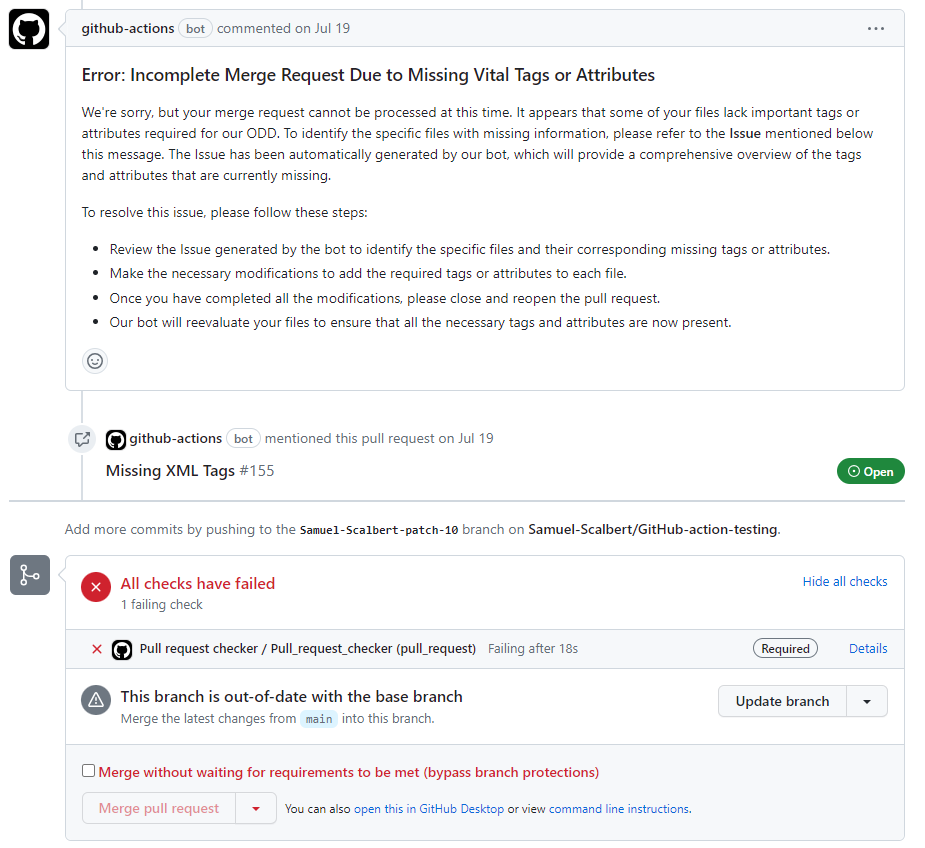
\includegraphics[width=0.75\linewidth]{schémas/gitaction_pr.png}
\caption{Exemple d'une demande de fusion refusée par GitHub Actions}
\label{fig:schémas14}
\end{figure}

\begin{figure}[H]
\centering
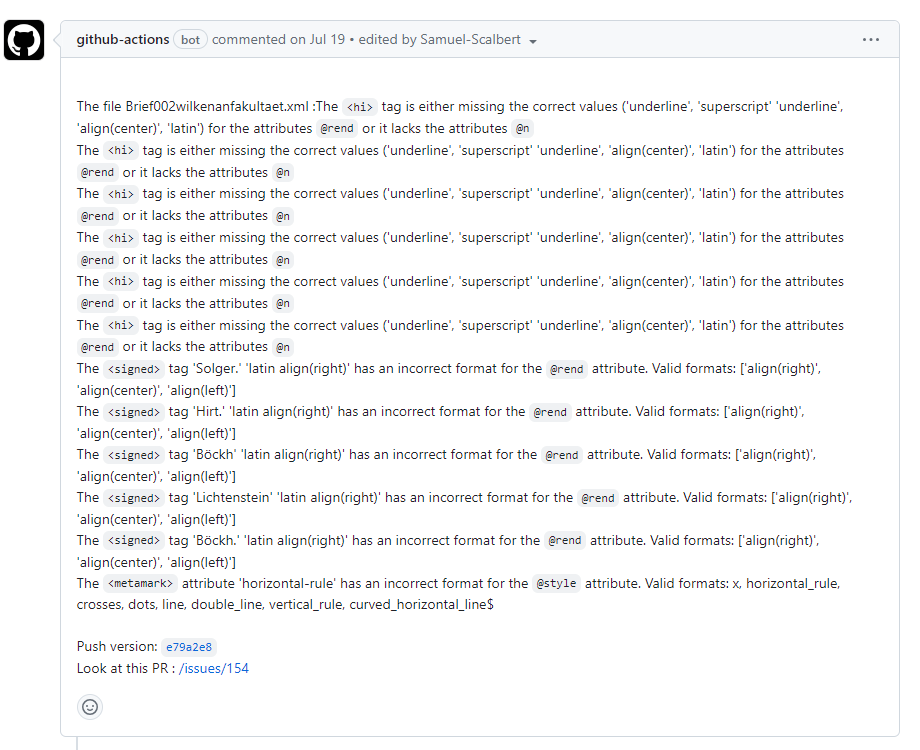
\includegraphics[width=0.75\linewidth]{schémas/gitactions_issue.png}
\caption{Exemple d'une \textit{issue} créée par GitHub Actions}
\label{fig:schémas15}
\end{figure}

Ce GitHub Action permet de vérifier rapidement et facilement si l'encodage du corpus correspond à notre ODD, évitant ainsi de nombreux problèmes. De plus, elle offre la possibilité à toute personne souhaitant soumettre son corpus à DiScholEd de vérifier directement son encodage, sans avoir à attendre l'approbation d'un membre de l'équipe DiScholEd.\\

Le dernier problème, après l'encodage des fichiers, était le \textit{design} de notre application.

\section{Un \textit{bundle} spécifique pour Discholed}

Nous avons souvent évoqué le \textit{bundle} de TEI Publisher et expliqué qu'il apporte des fonctionnalités essentielles, mais qu'il limite le \textit{design} général de l'application.

Il est possible de créer son propre \textit{bundle} à partir de celui disponible sur le \href{https://github.com/eeditiones/tei-publisher-components}{GitHub}\footnote{URL : https://github.com/eeditiones/tei-publisher-components} de TEI Publisher. Un \textit{bundle} spécialement développé pour notre application pourrait résoudre tous nos problèmes, mais cela nécessite une solide expertise en développement. Le seul inconvénient alors serait que notre \textit{bundle} ne recevrait plus les mises à jour.

En effet, en utilisant une version modifiée du \textit{bundle}, il faudrait le charger non plus depuis Internet, mais à partir des fichiers de l'application. Ainsi, notre \textit{bundle} ne serait plus mis à jour, nos éléments fonctionneraient, mais nous perdrions les nouvelles fonctionnalités développées par TEI Publisher et les correctifs de \textit{bugs}.
